\documentclass[sigconf, nonacm, screen]{acmart}
\usepackage[brazil]{babel}
\usepackage{microtype}
\usepackage{hyphenat}
\settopmatter{printccs=false}
\usepackage{graphicx}
\usepackage{soul}
\usepackage{balance}
\usepackage{listings}
\definecolor{islamicgreen}{rgb}{0.0, 0.56, 0.0}
\definecolor{light-gray}{gray}{.85}
\definecolor{codegray}{gray}{0.5}
\definecolor{richelectricblue}{rgb}{0.03, 0.57, 0.82}
\definecolor{red-violet}{rgb}{0.78, 0.08, 0.52}
\definecolor{patriarch}{rgb}{0.5, 0.0, 0.5}
\definecolor{red-brown}{rgb}{0.65, 0.16, 0.16}
\lstdefinestyle{mystyle}{
commentstyle=   \color{codegray},
keywordstyle=[1]\color{islamicgreen}\bfseries,
keywordstyle=[2]\color{patriarch},
keywordstyle=[3]\color{red-brown},
identifierstyle=\color{richelectricblue},
stringstyle=    \color{red-violet},
numberstyle=\tiny\color{codegray}, %numeração de linhas
basicstyle          = \ttfamily\footnotesize,
frame               = single,
rulecolor			= \color{codegray},
columns             = fullflexible,
breakatwhitespace   = false,
breaklines          = true,
keepspaces          = true,
showspaces          = false,
showstringspaces    = false,
inputencoding       = utf8,
extendedchars       = true,
literate            =
{á}{{\'a}}1 {é}{{\'e}}1 {í}{{\'i}}1 {ó}{{\'o}}1 {ú}{{\'u}}1
{Á}{{\'A}}1 {É}{{\'E}}1 {Í}{{\'I}}1 {Ó}{{\'O}}1 {Ú}{{\'U}}1
{à}{{\`a}}1 {è}{{\`e}}1 {ì}{{\`i}}1 {ò}{{\`o}}1 {ù}{{\`u}}1
{À}{{\`A}}1 {È}{{\'E}}1 {Ì}{{\`I}}1 {Ò}{{\`O}}1 {Ù}{{\`U}}1
{ä}{{\"a}}1 {ë}{{\"e}}1 {ï}{{\"i}}1 {ö}{{\"o}}1 {ü}{{\"u}}1
{Ä}{{\"A}}1 {Ë}{{\"E}}1 {Ï}{{\"I}}1 {Ö}{{\"O}}1 {Ü}{{\"U}}1
{â}{{\^a}}1 {ê}{{\^e}}1 {î}{{\^i}}1 {ô}{{\^o}}1 {û}{{\^u}}1
{Â}{{\^A}}1 {Ê}{{\^E}}1 {Î}{{\^I}}1 {Ô}{{\^O}}1 {Û}{{\^U}}1
{œ}{{\oe}}1 {Œ}{{\OE}}1 {æ}{{\ae}}1 {Æ}{{\AE}}1 {ß}{{\ss}}1
{ç}{{\c c}}1 {Ç}{{\c C}}1 {ø}{{\o}}1 {å}{{\r a}}1 {Å}{{\r A}}1
{€}{{\EUR}}1 {£}{{\pounds}}1 {ã}{{\~a}}1 {Ã}{{\~A}}1,
showtabs=false,
tabsize=2,
numbers=left,
numbersep=5pt,
aboveskip=5pt,
belowskip=15pt,
%captionpos=b
}
\lstset{style=mystyle}
\renewcommand{\figureautorefname}{Figura}
\renewcommand{\tableautorefname}{Tabela}
\renewcommand{\lstlistingname}{Listagem}
\newcommand{\no}[0]{\textsuperscript{\b{o}}}
\newcommand{\red}[1]{\textbf{\color{ACMRed}#1}}
\newcommand{\blue}[1]{\textbf{\color{ACMBlue}#1}}
%========================================
% Latex font sizes
% command           10pt    11pt    12pt
% \tiny             5       6       6
% \scriptsize       7       8       8
% \footnotesize     8       9       10
% \small            9       10      10.95
% \normalsize       10      10.95   12
% \large            12      12      14.4
% \Large            14.4    14.4    17.28
% \LARGE            17.28   17.28   20.74
% \huge             20.74   20.74   24.88
% \Huge             24.88   24.88   24.88

% Picture: h=here, t=top, b=bottom, p=(page of float), ex.: \begin{figure}[ht]
%========================================

\begin{document}

\title{Comparação de modelos de redes neurais artificiais CNN e MLP, para um caso de teste de reconhecimento ótico de caracteres}

\begin{abstract}
Algumas topologias e parâmetros diferentes para uma rede neural artificial convolucional (CNN) são comparados com um modelo do tipo Perceptron Multi-Camadas (MLP), utilizando o dataset MNIST para reconhecimento ótico de caracteres. Redes neurais têm sido usadas para resolver uma grande variedade de tarefas que são difíceis de resolver utilizando programação baseada em regras comuns, incluindo visão computacional e reconhecimento de voz \cite{TF}. Este trabalho utilizou a biblioteca TensorFlow para comparar alguns modelos CNN e dentre eles selecionar os dois com melhor acurácia, e também foi comparado com o modelo MLP.
\end{abstract}

%%
%% Keywords. The author(s) should pick words that accurately describe the work being presented.
\settopmatter{printfolios=true}
\keywords{Aprendizado de máquina, Redes neurais artificiais, Inteligência artificial, Computação científica}

%%
%% This command processes the author and affiliation and title information and builds the first part of the formatted document.
\maketitle

%========================================
\section{Introdução}
\label{sec:introduction}

Redes neurais artificias são algoritmos que tentam de alguma forma se assemelhar a neurônios biológicos, e usam alguns conceitos como sinapses e transmissão de sinais processados para outros neurônios conectados. Os sinais são representados na forma de números, e a saída de um neurônio é o resultado de um cálculo feito por uma função não linear que leva em consideração a soma das entradas do neurônio. Tipicamente neurônios possuem pesos e \textit{bias} que precisam ser ajustados em uma etapa anterior conhecida como treinamento. Os pesos aumentam ou diminuem a intensidade do sinal na conexão. Neurônios podem ser configurados para possuírem um limiar aonde o sinal é enviado somente se ultrapassar aquele limiar.

\begin{figure}[ht]
	\centering
	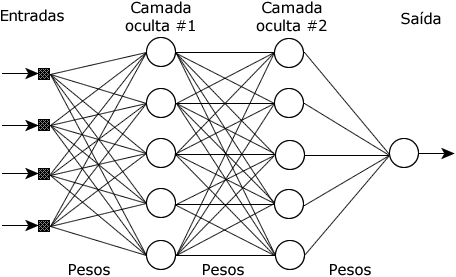
\includegraphics[width=0.9\linewidth]{img/mlp}
	\caption{Rede MLP.}
	\label{fig:mlp}
\end{figure}

\begin{figure}[ht]
	\centering
	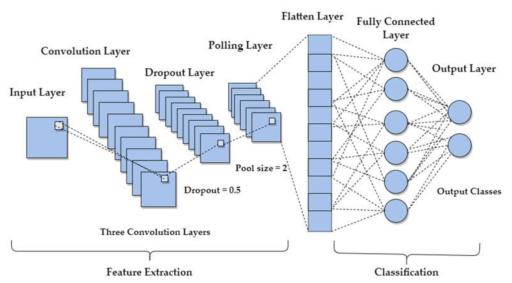
\includegraphics[width=\linewidth]{img/cnn}
	\caption{Rede CNN.}
	\label{fig:cnn}
\end{figure}

A \autoref{fig:mlp} mostra uma rede neural artificial usando a topologia MLP (Perceptron Multi-Camadas) que possui uma camada de entrada, duas camadas ocultas, e uma de saída com um neurônio. A \autoref{fig:cnn} mostra um exemplo usando a topologia CNN (rede neural convolucional) que inclui camadas de extração de recursos como convolução, \textit{dropout}, \textit{pooling}, e \textit{flatten}.

\begin{figure}[ht]
	\centering
	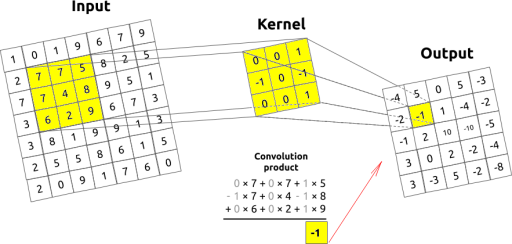
\includegraphics[width=\linewidth]{img/convolucao}
	\caption{Convolução.}
	\label{fig:convolucao}
\end{figure}

Na rede CNN um exemplo de camada de convolução é mostrado na \autoref{fig:convolucao}, e consiste em usar um kernel de convolução na camada de entrada para produzir um tensor de saídas.

\begin{figure}[ht]
	\centering
	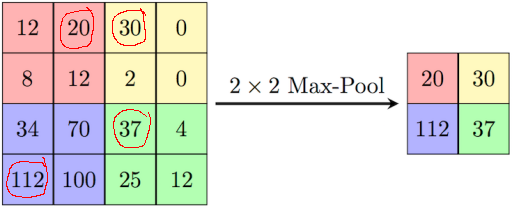
\includegraphics[width=0.9\linewidth]{img/pool}
	\caption{\textit{Pooling}.}
	\label{fig:pool}
\end{figure}

Um exemplo de \textit{pooling} é mostrado na \autoref{fig:pool} e consiste em reduzir a amostra de entrada ao longo de suas dimensões espaciais (altura e largura) tomando o valor máximo em uma janela de entrada para cada canal de entrada. A janela é deslocada a passos largos ao longo de cada dimensão.

\begin{figure}[ht]
	\centering
	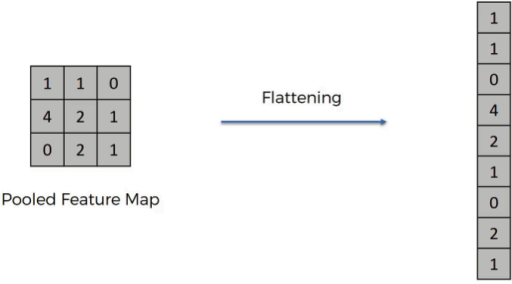
\includegraphics[width=0.8\linewidth]{img/flat}
	\caption{Flattening.}
	\label{fig:flatt}
\end{figure}

Um exemplo de \textit{fattening} é mostrado na \autoref{fig:flatt} e consiste em mudar o formato dos dados e deixá-los achatados.

\begin{figure}[ht]
	\centering
	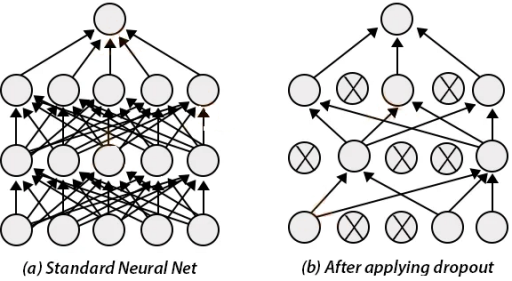
\includegraphics[width=0.9\linewidth]{img/dropout}
	\caption{Dropout.}
	\label{fig:dropout}
\end{figure}

Um exemplo de \textit{dropout} é mostrado na \autoref{fig:dropout} e consiste em desativar alguns neurônios durante o treinamento, para tentar reduzir o \textit{overfitting}.

\begin{figure}[ht]
	\centering
	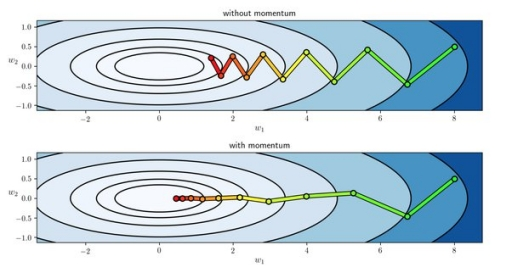
\includegraphics[width=0.9\linewidth]{img/momentum}
	\caption{Momentum.}
	\label{fig:momentum}
\end{figure}

Alguns parâmetros que podem ser usados durante o treinamento são o Momentum (\autoref{fig:momentum}) e a regularização (\autoref{fig:regularizacao}). O momentum é utilizado quando se usa o algoritmo de otimização de gradiente descendente, onde é possível que a superfície que a equação descreve seja complexa e com vários mínimos locais, dificultando a obtenção do mínimo global. Neste caso pode-se usar o termo de momentum para aumentar o tamanho dos passos dados em direção ao mínimo, desta forma tentando saltar os mínimos locais.

\begin{figure}[ht]
	\centering
	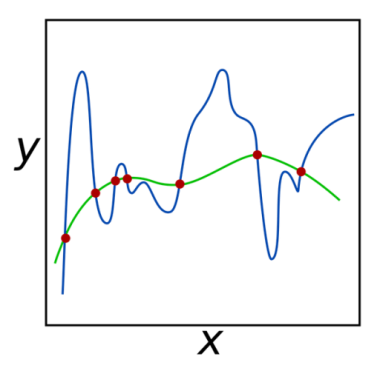
\includegraphics[width=0.5\linewidth]{img/regularizacao}
	\caption{Regularização.}
	\label{fig:regularizacao}
\end{figure}

A regularização pode ser utilizada para evitar o \textit{overfitin}g dos dados, estabelecendo um limite para os pesos evitando a saturação de sinapses.




%========================================
\section{Classificação de imagens}
\label{sec:descricao}

O dataset MNIST (\textit{Modified National Institute of Standards and Technology}) consiste em um grande conjunto de dígitos escritos à mão digitalizados e classificados, é usualmente utilizado para treinamento de sistemas de processamento de imagens, e também em aprendizado de máquina. Possui 60 mil imagens para treinamento e 10 mil para teste, e cada imagem tem 20x28 pixels usando níveis de cinza. A Figura \ref{fig:mnist} mostra uma representação de uma imagem e a correspondente rede neural artificial.

\begin{figure}[ht]
	\centering
	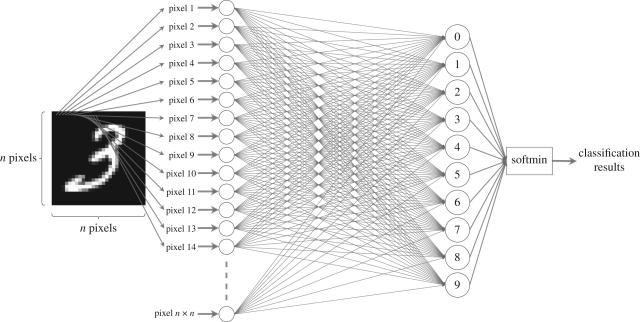
\includegraphics[width=\linewidth]{img/mnist2}
	\caption{Dataset MNIST e rede neural artificial. Fonte:royalsocietypublishing.org.}
	\label{fig:mnist}
\end{figure}




%========================================
\section{Implementação}
\label{sec:implementacoes}

Para a rede CNN, a implementação da primeira topologia mostrada na \autoref{lst:topo1} foi feita usando a biblioteca TensorFlow e foi definida como mostrado na \autoref{fig:topo} com uma camada de entrada seguida por uma de convolução, uma de \textit{pooling}, uma de \textit{flattening}, uma \textit{dense} (camada totalmente conectada e o tipo mais comum de camada usado em modelos perceptron multicamadas), uma \textit{dropout}, e finalmente uma camada de saída).

\begin{lstlisting}[language=Python,label=lst:topo1,caption={Topologia 1 - definição das camadas da rede neural artificial.}]
model = Sequential()
model.add(
    Conv2D(
        32,  # number or filters (output)
        (3, 3),  # kernel size
        activation="relu",
        kernel_initializer="he_uniform",
        input_shape=in_shape))  # (28, 28, 1)
model.add(MaxPool2D((2, 2)))
model.add(Flatten())
model.add(Dense(100, activation="relu",
          kernel_initializer="he_uniform"))
model.add(Dropout(0.5))
model.add(Dense(n_classes, activation="softmax"))
\end{lstlisting}

\begin{figure}[ht]
	\centering
	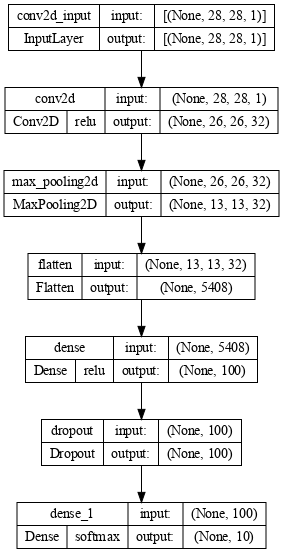
\includegraphics[width=0.6\linewidth]{img/topo1}
	\caption{Topologia 1.}
	\label{fig:topo}
\end{figure}

A função de ativação usada foi a ReLU (\autoref{fig:relu}) que retorna o próprio valor se ele for negativo, ou então zero se for negativo. Como ela retorna zero para valores negativos, tende a "apagar" alguns neurônios durante o treinamento. Da mesma forma, valores positivos podem "explodir" durante o treinamento pois não impõe um valor limite.

\begin{figure}[ht]
	\centering
	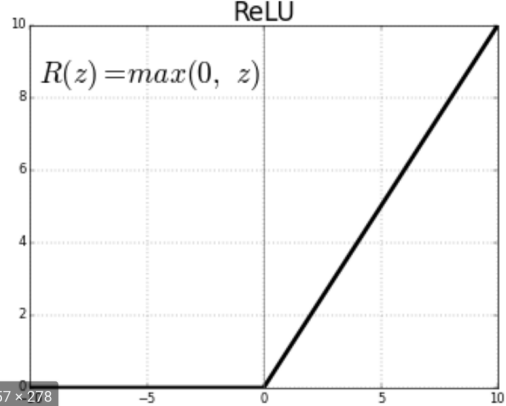
\includegraphics[width=0.6\linewidth]{img/relu}
	\caption{Função de ativação ReLU.}
	\label{fig:relu}
\end{figure}

O argumento \texttt{kernel\_initializer} define os pesos aleatórios iniciais das camadas de neurônios, durante o treinamento. O valor \texttt{he\_uniform} faz com que sejam utilizadas amostras de uma distribuição uniforme onde os limites são dados por: $ limit = \sqrt{6 \over \texttt{fan\_in}} $ onde \texttt{fan\_in} é a quantidade de unidades de entrada no tensor de peso.

O argumento {input\_shape} é usado para definir a camada de entrada. A função \texttt{MaxPool2D} define o \textit{pooling}, \texttt{Flatten} achata os dados, \texttt{Dense} define uma camada totalmente conectada de neurônios, \texttt{Dropout} faz com que alguns neurônios sejam "desativados" para tentar evitar o \textit{overfitting}, e finalmente na camada de saída temos a ativação \texttt{softmax} que converte um vetor de valores em uma distribuição probabilística sendo que os elementos do vetor de saída estão no intervalo (0,1) e somam 1.

\begin{lstlisting}[language=Python,label=lst:ctre1,caption={Topologia 1 - configuração do modelo de treinamento}]
model.compile(optimizer='adam',
              loss='sparse_categorical_crossentropy',
              metrics=['accuracy'])
\end{lstlisting}

A definição do modelo de treinamento é mostrado na \autoref{lst:ctre1}. O otimizador \texttt{adam} é um algoritmo que implementa o método estocástico de gradiente descendente baseado na estimativa adaptativa de momentos de primeira e de segunda ordem. O parâmetro \texttt{sparse\_categorical\_crossentropy} define o cálculo da perda de entropia cruzada entre os rótulos e as previsões, quando há duas ou mais classes de rótulos. A métrica \texttt{accuracy} calcula a frequência com que as previsões são iguais aos rótulos.

\begin{lstlisting}[language=Python,label=lst:trei1,caption={Topologia 1 - treinamento do modelo}]
history = model.fit(x_train_norm,
                    y_train,
                    epochs=100,
                    batch_size=128,
                    validation_data=(x_test_norm, y_test),
                    verbose=0)
\end{lstlisting}

A definição e o treinamento são mostrados na \autoref{lst:trei1}. A quantidade de épocas de treinamento foi definida como 100. O \texttt{batch\_size} define o número de amostras por atualização de gradiente (128). O \texttt{validation\_data} são os dados sobre os quais é feita a validação da perda e quaisquer métricas do modelo no final de cada época.

\begin{figure}[ht]
	\centering
	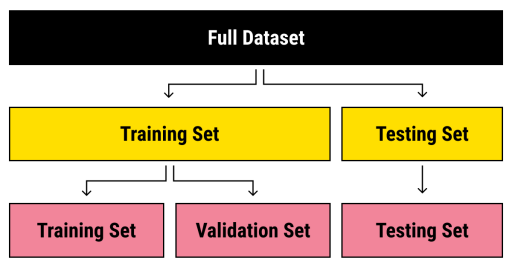
\includegraphics[width=0.9\linewidth]{img/trai-vali-test}
	\caption{Divisão do dataset em conjuntos de treinamento, validação, e teste.}
	\label{fig:tvt}
\end{figure}

A \autoref{fig:tvt} mostra a divisão usual do conjunto de dados em Treinamento, Validação, e Teste. Para este trabalho, no entanto, como a intenção era avaliar a validação, somente dois conjuntos foram utilizados, um de Treino e um único de Validação/Teste.





%========================================
\section{Análise}
\label{sec:analise}

\begin{figure}[ht]
	\centering
	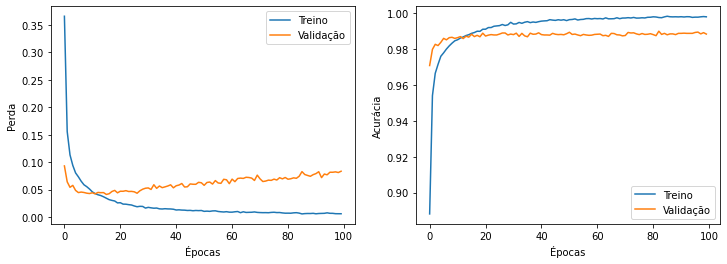
\includegraphics[width=\linewidth]{img/perd_acur_1}
	\caption{Perda e acurácia para a topologia 1.}
	\label{fig:perdacur1}
\end{figure}

A \autoref{fig:perdacur1} mostra os gráficos de perda e acurácia para a Topologia 1 descrita na seção anterior. A acurácia obtida foi de 0.988. A perda usando dados de validação (teste) tem a tendência de ir aumentando ao longo das épocas, tendência inversa do treinamento. As próximas topologias são uma variação desta primeira.

\begin{figure}[ht]
	\centering
	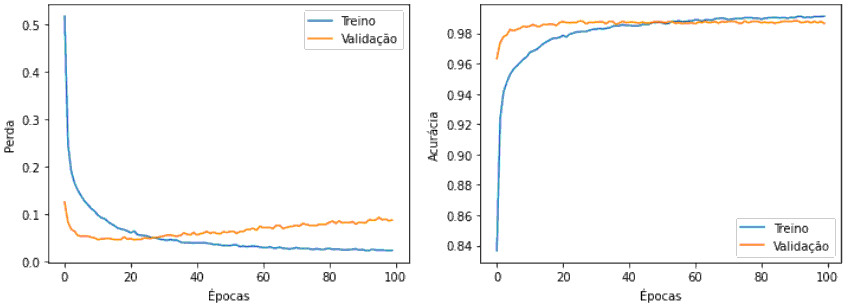
\includegraphics[width=\linewidth]{img/perd_acur_2}
	\caption{Perda e acurácia para a topologia 2.}
	\label{fig:perdacur2}
\end{figure}

A \autoref{fig:perdacur1} mostra os gráficos de perda e acurácia para a Topologia 2. A diferença entre a topologia 1 e 2 está na camada escondida que foi reduzida de 100 neurônios para 50. A acurácia obtida foi de 0.987, um pouco menor que a topologia anterior. O treino demora um pouco mais para chegar no mínimo de perda, quando comparado com a topologia 1.

\begin{figure}[ht]
	\centering
	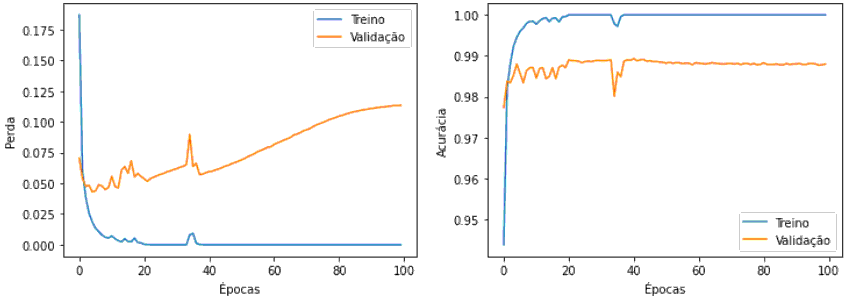
\includegraphics[width=\linewidth]{img/perd_acur_3}
	\caption{Perda e acurácia para a topologia 3.}
	\label{fig:perdacur3}
\end{figure}

A \autoref{fig:perdacur3} mostra os gráficos de perda e acurácia para a Topologia 3. Nesta topologia a camada Dropout foi eliminada. A acurácia obtida foi de 0.988, similar à primeira topologia, porém a perda durante a validação é grande.

\begin{figure}[ht]
	\centering
	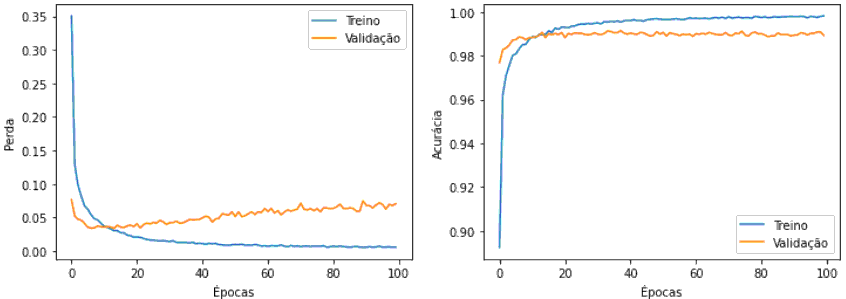
\includegraphics[width=\linewidth]{img/perd_acur_4}
	\caption{Perda e acurácia para a topologia 4.}
	\label{fig:perdacur4}
\end{figure}

A \autoref{fig:perdacur4} mostra os gráficos de perda e acurácia para a Topologia 4. Nesta topologia o tamanho do kernel foi aumentado de 3x3 para 5x5. A acurácia obtida foi de 0.989, maior do que as topologias anteriores.

\begin{figure}[ht]
	\centering
	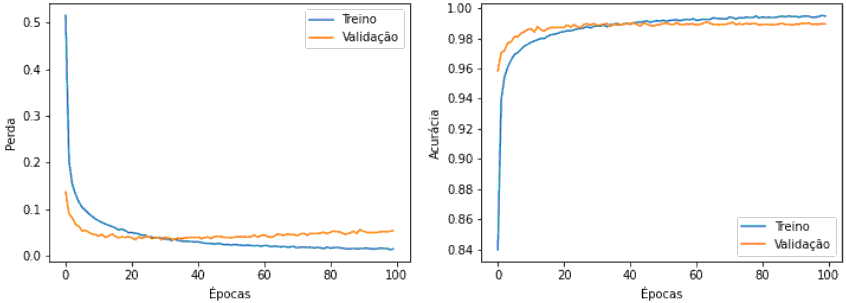
\includegraphics[width=\linewidth]{img/perd_acur_5}
	\caption{Perda e acurácia para a topologia 5.}
	\label{fig:perdacur5}
\end{figure}

A \autoref{fig:perdacur5} mostra os gráficos de perda e acurácia para a Topologia 5. Nesta topologia o Maxpool (pool) passou de 2x2 para 5x5. Assim como a topologia anterior (4), aumentou a acurácia com relação às primeiras topologias.

\begin{figure}[ht]
	\centering
	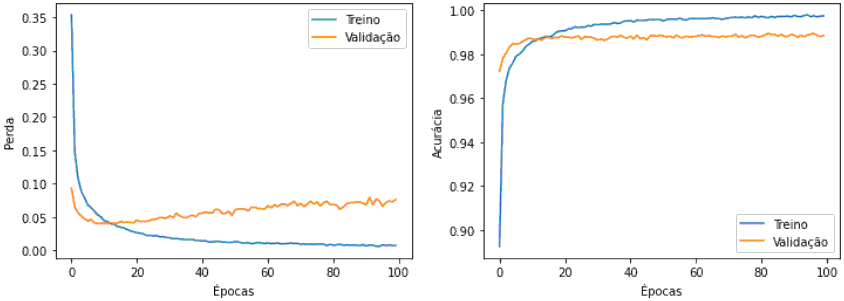
\includegraphics[width=\linewidth]{img/perd_acur_6}
	\caption{Perda e acurácia para a topologia 6.}
	\label{fig:topo6}
\end{figure}

A \autoref{fig:topo6} mostra os gráficos de perda e acurácia para a Topologia 6. Nesta topologia a quantidade de filtros de saída na camada convolucional (Conv2D) passou de 32 para 16. A acurácia não aumentou, como aconteceu com a topologia anterior.

\begin{figure}[ht]
	\centering
	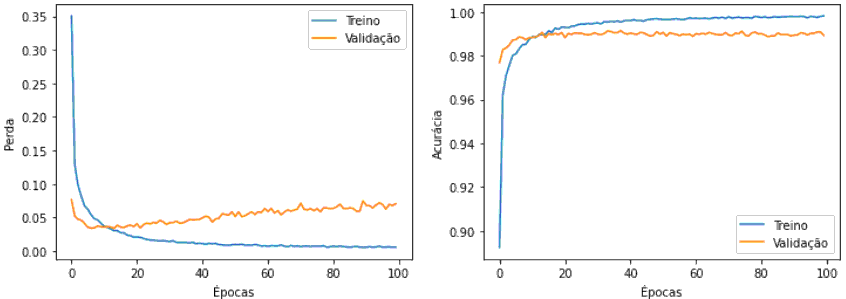
\includegraphics[width=\linewidth]{img/perd_acur_4}
	\caption{Perda e acurácia para a topologia 4.}
	\label{fig:topo4}
\end{figure}

A \autoref{fig:perdacur4} mostra os gráficos de perda e acurácia para a Topologia 7. Nesta topologia foi alterado de 32 para 16 filtros em Conv2D, e de 100 para 30 neurônios na camada intermediária (Dense). A acurácia piorou.

\begin{table}
\small
\caption{Acurácias obtidas nos experimentos. Os maiores valores estão em vermelho.}
\label{tab:acur}
\begin{tabular}{cc}\toprule
\textbf{Topologia}      & \textbf{Acurácia} \\
\hline\vspace{-9pt}     & \\
\textbf{1}              &  0.988 \\
\textbf{2}              &  0.987 \\
\textbf{3}              &  0.988 \\
\textbf{4}              &  \red{0.989} \\
\textbf{5}              &  \red{0.989} \\
\textbf{6}              &  0.988 \\
\textbf{7}              &  0.985 \\
\bottomrule
\end{tabular}
\end{table}

A \autoref{tab:acur} mostras as acurácias obtidas nos experimentos realizados, onde foram usados topologias e parâmetros diferentes. As duas melhores acurácias foram obtidas nas topologias 4 e 5. Para estas duas, foram feitos os gráficos de matriz de confusão, e um heatmap mostrando um teste de McNemar para as duas topologias.

\begin{figure}[ht]
	\centering
	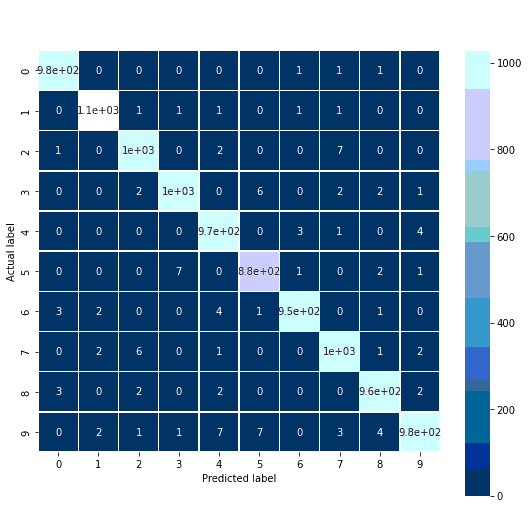
\includegraphics[width=0.8\linewidth]{img/confu4}
	\caption{Matriz de confusão para a topologia 4.}
	\label{fig:confu4}
\end{figure}

A \autoref{fig:confu4} mostra a matriz de confusão comparando a predição com o valor real, para a topologia 4. Como a acurácia foi relativamente alta, a linha diagonal concentra a maior quantidade de predições corretas.

\begin{figure}[ht]
	\centering
	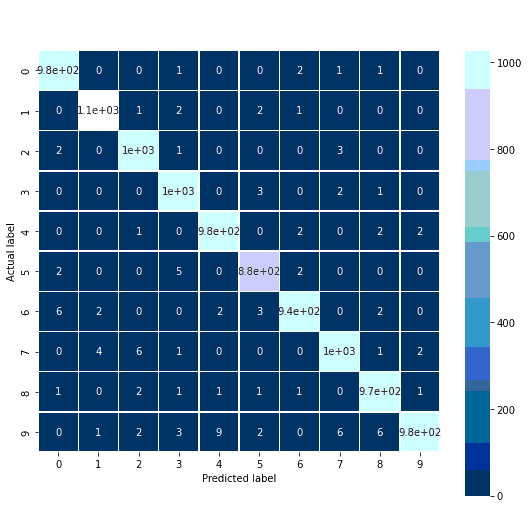
\includegraphics[width=0.8\linewidth]{img/confu5}
	\caption{Matriz de confusão para a topologia 5.}
	\label{fig:confu5}
\end{figure}

A \autoref{fig:confu5} mostra a matriz de confusão comparando a predição com o valor real, para a topologia 5. Da mesma forma que para a topologia 4, como a acurácia foi relativamente alta, a linha diagonal concentra a maior quantidade de predições corretas.


\begin{figure}[ht]
	\centering
	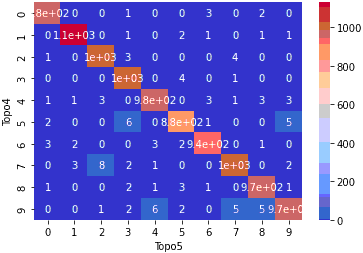
\includegraphics[width=0.8\linewidth]{img/mnem}
	\caption{Teste de McNemar para os dois melhores modelos (4 e 5).}
	\label{fig:mnem}
\end{figure}

A \autoref{fig:mnem} mostra o teste de McNemar comparando a predição com o valor real, para os dois melhores modelos (4 e 5). Este gráfico também mostra na linha diagonal os valores relativamente altos de predições corretas.


\begin{figure}[ht]
	\centering
	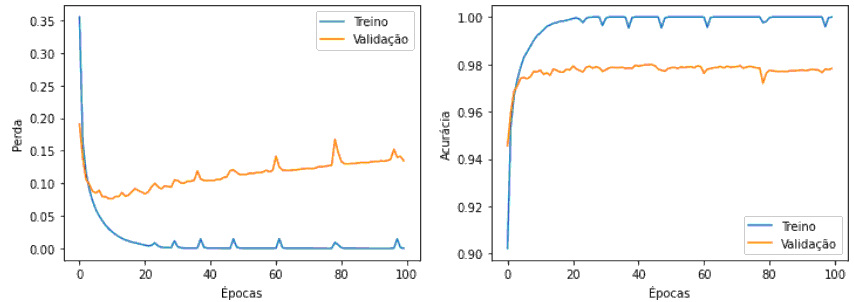
\includegraphics[width=0.8\linewidth]{img/mlpresult}
	\caption{Resultado para a topologia MLP.}
	\label{fig:mlpresult}
\end{figure}

A \autoref{fig:mlpresult} mostra os gráficos de perda e acurácia para a Topologia MLP. Esta topologia mostrou que durante o treinamento a acurácia foi equivalente à rede CNN, porém para os dados de treinamento a acurácia foi pior.


\begin{figure}[ht]
	\centering
	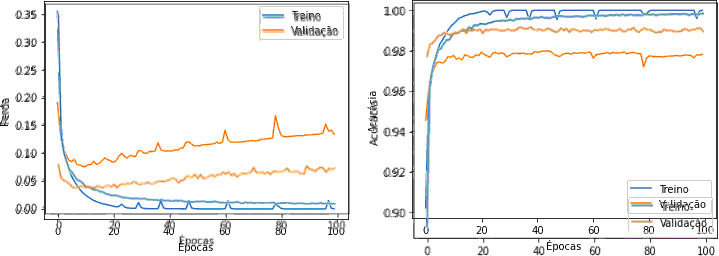
\includegraphics[width=0.8\linewidth]{img/mlpcnn}
	\caption{Sobreposição dos gráficos MLP e CNN.}
	\label{fig:mlpcnn}
\end{figure}

A \autoref{fig:mlpcnn} mostra dois gráficos sobrepostos, MLP e CNN. As curvas de treinamento em azul estão próximas, porém as de validação estão distantes, mostrando uma maior acurácia da topologia CNN.


%========================================
\section{Comentários finais}
\label{sec:conclusao}

O trabalho mostrou algumas topologias para a rede CNN e uma topologia MLP, e fez comparações entre elas. O dataset MNIST foi escolhido, e a biblioteca TensorFlow foi utilizada. A comparação CNN x MLP mostrou uma maior acurácia para a rede CNN utilando os dados de validação. Nas topologias CNN não houve grande variação na acurácia, porém as duas topologias com maior acurácia foram selecionadas e comparadas.





%========================================
\balance
\nocite{*}
\bibliographystyle{ACM-Reference-Format}
\bibliography{references.bib}
\label{chp:bibl}

\end{document}
\endinput
%%
%% End of file.